\documentclass{beamer}
\usepackage[utf8]{inputenc}
\usetheme{default}
\usecolortheme{seagull}
\setbeamertemplate{navigation symbols}{}

\title{AI and Large Language Model Chatbots for Real-World Businesses}
\author{Tero Keski-Valkama}
\date{\today}
\titlegraphic{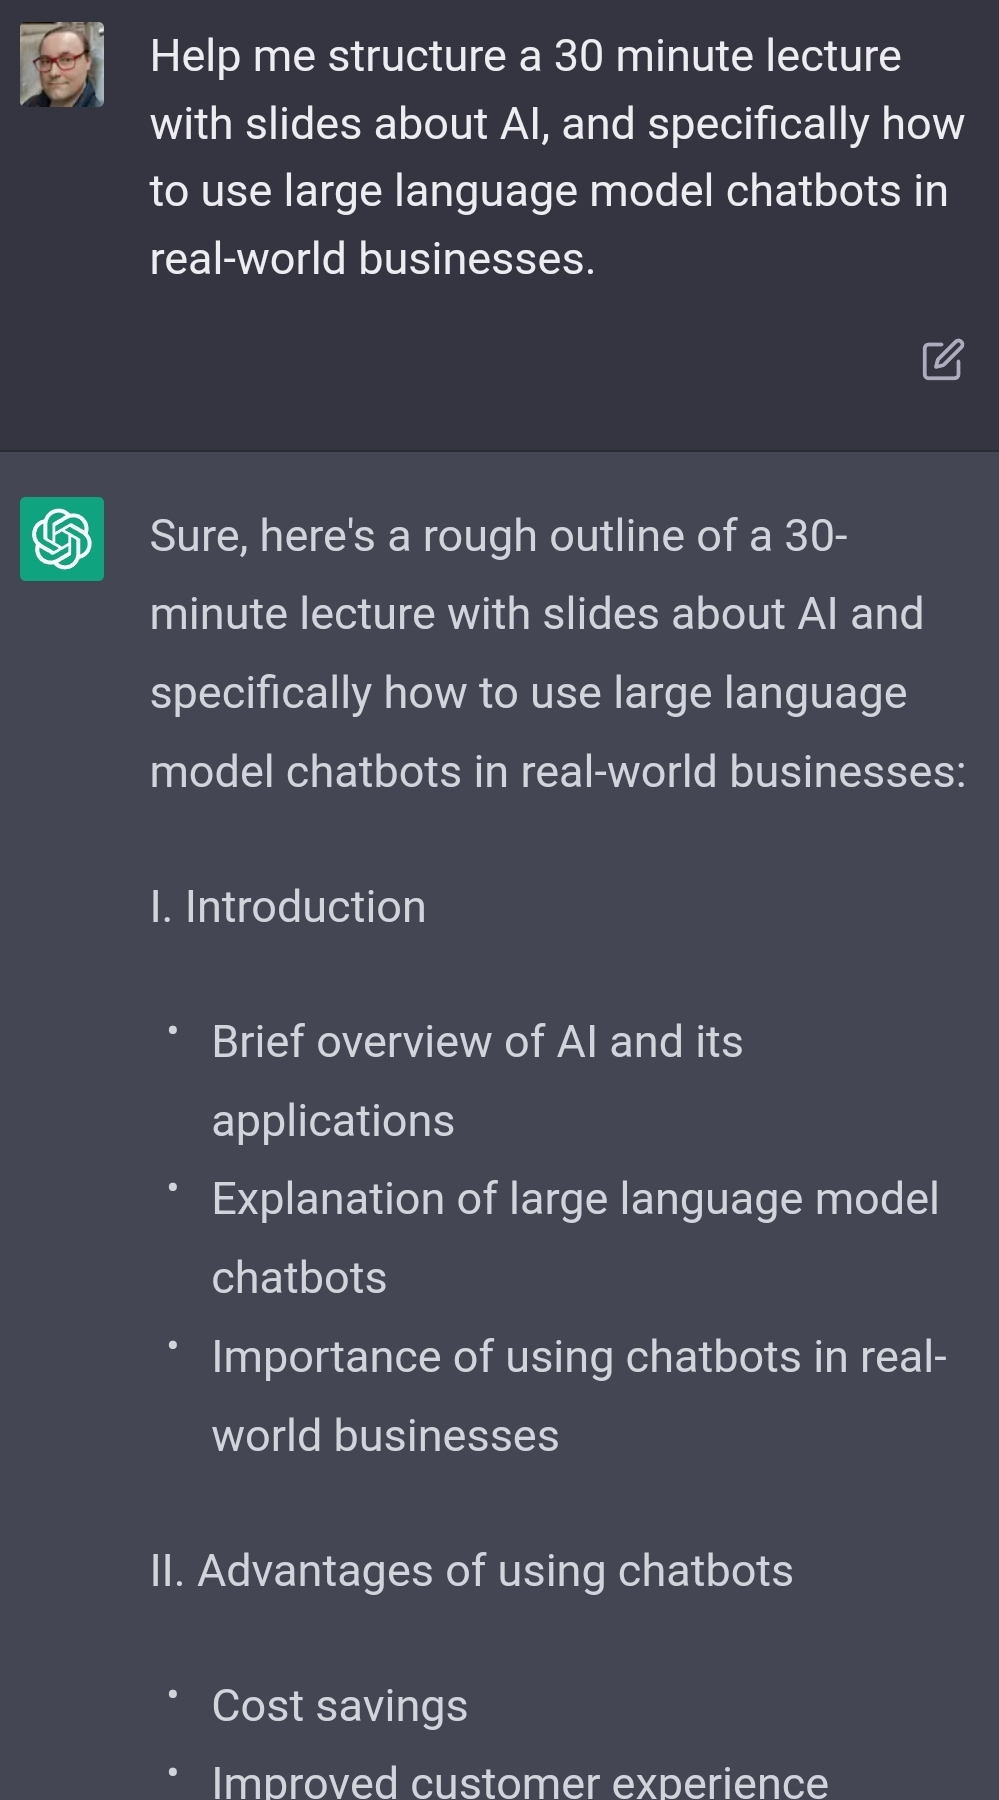
\includegraphics[height=4cm]{chatgpt_help.jpg}\hspace{0.3cm}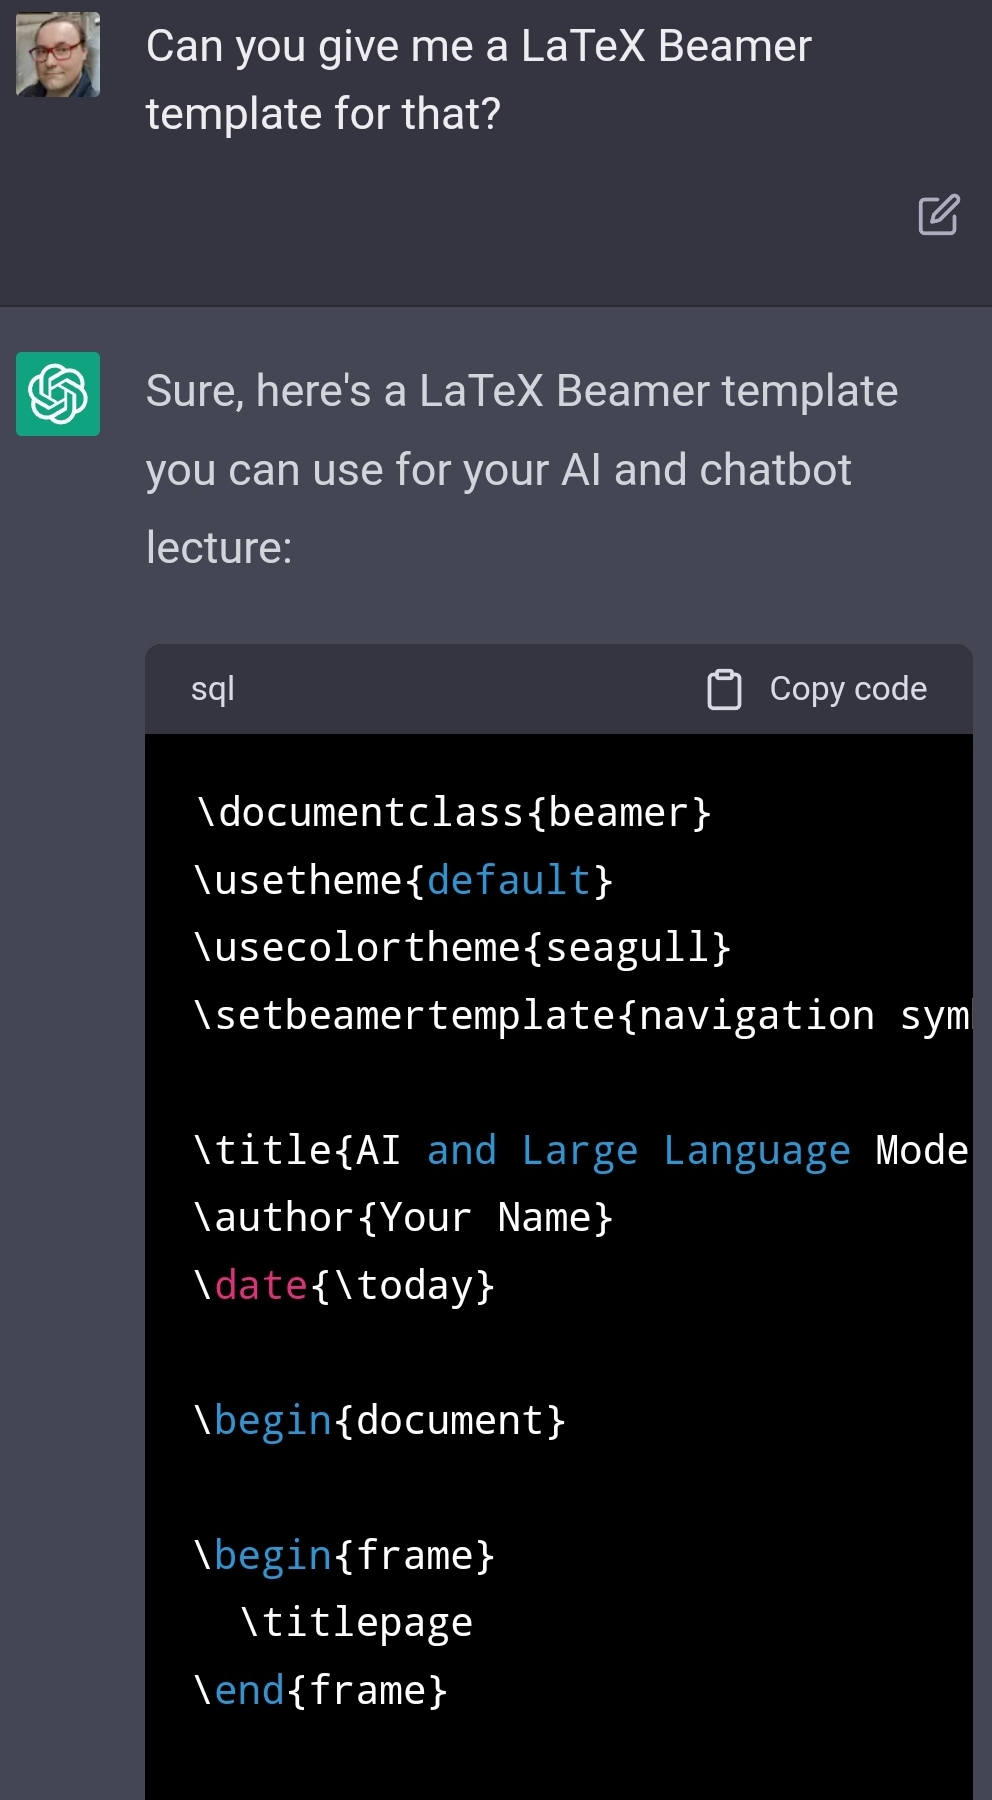
\includegraphics[height=4cm]{chatgpt_help_latex.jpg}
\hspace{0.3cm}
\includegraphics[height=4cm]{tero.jpg}}

\begin{document}

\begin{frame}
  \titlepage
\end{frame}

\section{Introduction}
\begin{frame}{Introduction: Tero Keski-Valkama}
  \begin{itemize}
    \item Tero Keski-Valkama is an AI practitioner with over 20 years of experience spanning four countries, currently living in Spain.
    \item Worked with machine vision, complex control, SLAM, sensor fusion, semantic web, perceptrons, genetic algorithms, simulated annealing, SVMs, gradient boosting, deep learning, deep reinforcement learning, GANs, CNNs, Transformers, \textbf{LLMs}, \textbf{AGI}, embodiment, meta-learning, ...
    \item Robotics, pre-LLM chatbots, \textbf{LLM chatbots}, facial emotion recognition, automatic mapping, logistics, supply chain, ...
    \item He has authored over 20 patents in the topic among countless other publications.
    \item Authored the first correct open source Google WaveNet implementation, the first communist AI, cofounded the second largest recurring AI event in Finland (AI Morning), ...
  \end{itemize}
\end{frame}

\section{Why Is This a Big Deal?}
\begin{frame}{Why Is This a Big Deal?}
  \textbf{Chatbots} is a misnomer – They don't just chat. They can control other machines, adapt/learn, and most importantly, they integrate together societies of people and machines. They are already as intelligent as humans in many important topics, and very soon surpass humans in every cognitive task.

  The \textbf{Technological Singularity} has started, and along it the societies are now waking up to a sudden and extreme appetite for data, knowledge, network connectivity and chips.

  \vspace{0.2cm}

  \begin{quote}
   ``The fabric tunnel that stretched out behind it was a \textbf{'camera tunnel...'} The shredded fragments of books and magazines flew down the tunnel like leaves in a tornado, twisting and tumbling. The inside of the fabric was stiched with thousands of tiny cameras. The shreds were being photographed again and again, from every angle and orientation, till finally the torn leaves dropped into a bin just in front of Robert.''

   - Vernor Vinge, Rainbows End
  \end{quote}

\end{frame}

\section{Inside Chatbots}
\begin{frame}{Inside Chatbots}
\center
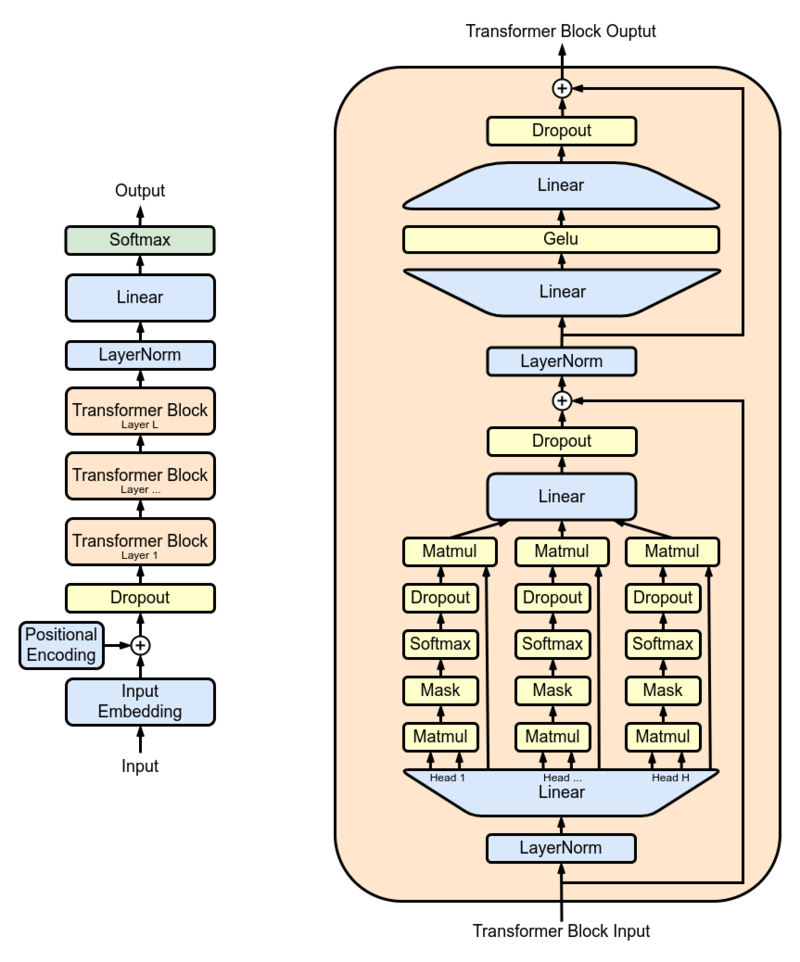
\includegraphics[height=9cm]{Full_GPT_architecture.png}
\end{frame}

\begin{frame}{Inside Chatbots}
So, Large Language Model (LLM) chatbots are based on a \textbf{Transformer} (or an RNN) architecture which is trained \textbf{autoregressively} on text (plus tricks). They only predict the next token (part-of-word) given what text comes before.

\vspace{0.5cm}

\textbf{\textit{So why are they so smart?}}

Turns out this task is \textbf{``AGI complete''}.

It is not possible to predict in general what words come next without understanding how people think and how the world works. That is indeed what these models have learned inside their basic structure.

How can we use their learned knowledge? Just train them to \textbf{emulate an assistant persona} which answers questions and performs tasks given to them. That is indeed what LLM chatbots are.
\end{frame}

\section{Using Chatbots in Business}
\begin{frame}{Using Chatbots in Business}
Chatbots know all of \textbf{Wikipedia} by heart but they don't know about your business. Whatever task you put them to perform, they need to know what you want.
  \begin{itemize}
    \item \textbf{``NEVER give money back for complaints!''}
  \end{itemize}
You need to be able to explain the task to the chatbot clearly and concisely. They are very smart, but they are not great at handling large amounts of text!

\vspace{0.5cm}

You can play around and test whether they are able to do what you want them to do in \textcolor{blue}{\href{https://chat.openai.com}{OpenAI ChatGPT frontend}}. When deploying you just use the \textcolor{blue}{\href{https://platform.openai.com/overview}{API}} they offer with Python language. The ChatGPT API costs a bit, but they tend to give some free credits for experimentation.
\end{frame}

\section{Future}
\begin{frame}{Future}
AIs will not match, they will \textbf{exceed all meaningful human cognitive capabilities} during this year.

What skills are important in the immediate future?
  \begin{itemize}
    \item \textbf{Clarity of thought}, \textbf{understanding} what is possible, and skill to \textbf{write} your knowledge, ideas and wants \textbf{clearly} to machines.
    \item \textbf{Empathy} and capability to understand the points of view of others, specifically of chatbots but also of other people. What don't they understand, and how to explain it to them better?
  \end{itemize}
\end{frame}

\end{document}
